\documentclass[tikz,border=10pt]{standalone}
\usepackage[T1]{fontenc}
\usepackage[sfdefault]{FiraSans}
\usepackage{tikz}
\usetikzlibrary{arrows.meta,positioning,calc,decorations.pathreplacing}
\definecolor{navy}{HTML}{003C6C}
\definecolor{navydeep}{HTML}{06294A}
\definecolor{ink}{HTML}{18293B}
\definecolor{muted}{HTML}{5B6B7C}
\definecolor{gold}{HTML}{FDC700}
\definecolor{amber}{HTML}{C98A00}
\definecolor{teal}{HTML}{0E7C9C}
\definecolor{coral}{HTML}{E4572E}
\definecolor{hairline}{HTML}{D9E1E9}
\definecolor{skyfill}{HTML}{E7F0F7}

\begin{document}
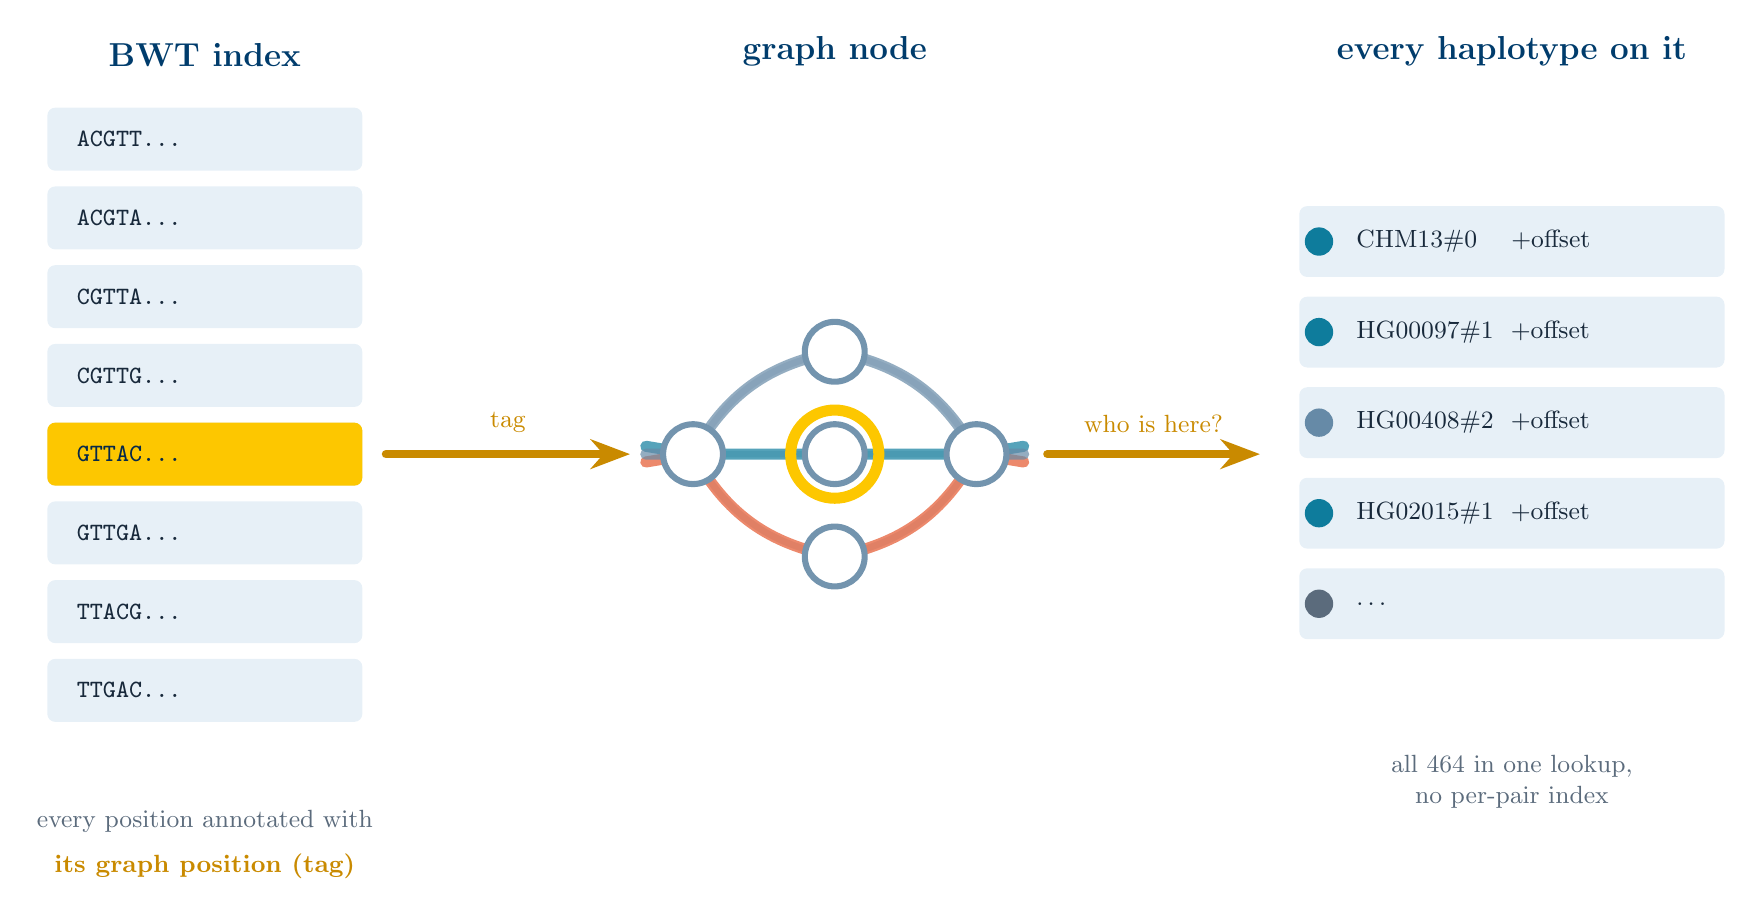
\begin{tikzpicture}[line cap=round, font=\normalsize]
  % BWT column
  \node[font=\large\bfseries, text=navy, anchor=south] at (2.0,9.1) {BWT index};
  \foreach \i/\s in {0/ACGTT\dots, 1/ACGTA\dots, 2/CGTTA\dots, 3/CGTTG\dots, 4/GTTAC\dots, 5/GTTGA\dots, 6/TTACG\dots, 7/TTGAC\dots}
    {\pgfmathsetmacro{\yy}{8.3-\i*1.0}
     \fill[skyfill, rounded corners=1mm] (0,\yy-0.4) rectangle (4.0,\yy+0.4);
     \node[anchor=west, font=\ttfamily\small, text=ink] at (0.25,\yy) {\s};}
  \fill[gold, rounded corners=1mm] (0,4.3-0.4) rectangle (4.0,4.3+0.4);
  \node[anchor=west, font=\ttfamily\small\bfseries, text=navydeep] at (0.25,4.3) {GTTAC\dots};
  \node[font=\small, text=muted, anchor=north] at (2.0,-0.1) {every position annotated with};
  \node[font=\small\bfseries, text=amber, anchor=north] at (2.0,-0.65) {its graph position (tag)};
  % arrow to node
  \draw[amber, line width=3pt, -{Stealth[length=5mm]}] (4.3,4.3) -- (7.4,4.3);
  \node[font=\small, text=amber, anchor=south] at (5.85,4.45) {tag};
  % graph node
  \node[font=\large\bfseries, text=navy, anchor=south] at (10.0,9.1) {graph node};
  \coordinate (n1) at (8.2,4.3); \coordinate (n2) at (10.0,4.3); \coordinate (n3) at (11.8,4.3);
  \coordinate (u) at (10.0,5.6); \coordinate (d) at (10.0,3.0);
  \draw[hairline, line width=2.4pt] (n1) -- (n2) -- (n3) (n1) to[bend left=25] (u) (u) to[bend left=25] (n3) (n1) to[bend right=25] (d) (d) to[bend right=25] (n3);
  \draw[teal, line width=4pt, opacity=0.7] (7.6,4.4) -- (n1) -- (n2) -- (n3) -- (12.4,4.4);
  \draw[coral, line width=4pt, opacity=0.7] (7.6,4.2) -- (n1) to[bend right=25] (d) to[bend right=25] (n3) -- (12.4,4.2);
  \draw[navy!60, line width=4pt, opacity=0.7] (7.6,4.3) -- (n1) to[bend left=25] (u) to[bend left=25] (n3) -- (12.4,4.3);
  \foreach \p in {n1,n2,n3,u,d} {\fill[white] (\p) circle (0.38); \draw[navy!55, line width=2.2pt] (\p) circle (0.38);}
  \draw[gold, line width=4pt] (n2) circle (0.56);
  % arrow to haplotypes
  \draw[amber, line width=3pt, -{Stealth[length=5mm]}] (12.7,4.3) -- (15.4,4.3);
  \node[font=\small, text=amber, anchor=south] at (14.05,4.45) {who is here?};
  % haplotype list
  \node[font=\large\bfseries, text=navy, anchor=south] at (18.6,9.1) {every haplotype on it};
  \foreach \i/\h/\c in {0/CHM13\#0 \ \ \ +offset/teal, 1/HG00097\#1 \ +offset/teal, 2/HG00408\#2 \ +offset/navy!60, 3/HG02015\#1 \ +offset/teal, 4/\dots/muted}
    {\pgfmathsetmacro{\yy}{7.0-\i*1.15}
     \fill[skyfill, rounded corners=1mm] (15.9,\yy-0.45) rectangle (21.3,\yy+0.45);
     \fill[\c] (16.15,\yy) circle (0.18);
     \node[anchor=west, font=\small, text=ink] at (16.5,\yy) {\h};}
  \node[font=\small, text=muted, anchor=north, align=center] at (18.6,0.6) {all 464 in one lookup,\\ no per-pair index};
\end{tikzpicture}
\end{document}
